%!TEX root = ../AliStrangeJets.tex

\section{Results and discussion}%
\label{sec:Results}

\subsection{Particles $\pT$-differential density}
\label{subsec:ParPtDensity}

For the strange hadrons discussed in this paper, the ratios of yields for particles and anti-particles are around one within the uncertainties, as expected at these collision energies in the mid-rapidity region.
Therefore, all the $\pT$-differential density shown in the following are reported after summing particles and anti-particles.
The different selections shown in the following have been introduced in section~\ref{sec:ParJetMatch}, inwhich also introduced the normalization method. 

Figure~\ref{fig:ppSpect} shown the $\kzero$, $\lmb + \almb$, $\X + \Ix$ and $\Om + \Mo$ $\pT$-differential density distributions in \pp collisions.


\begin{figure}[!ht]
	\begin{center}
		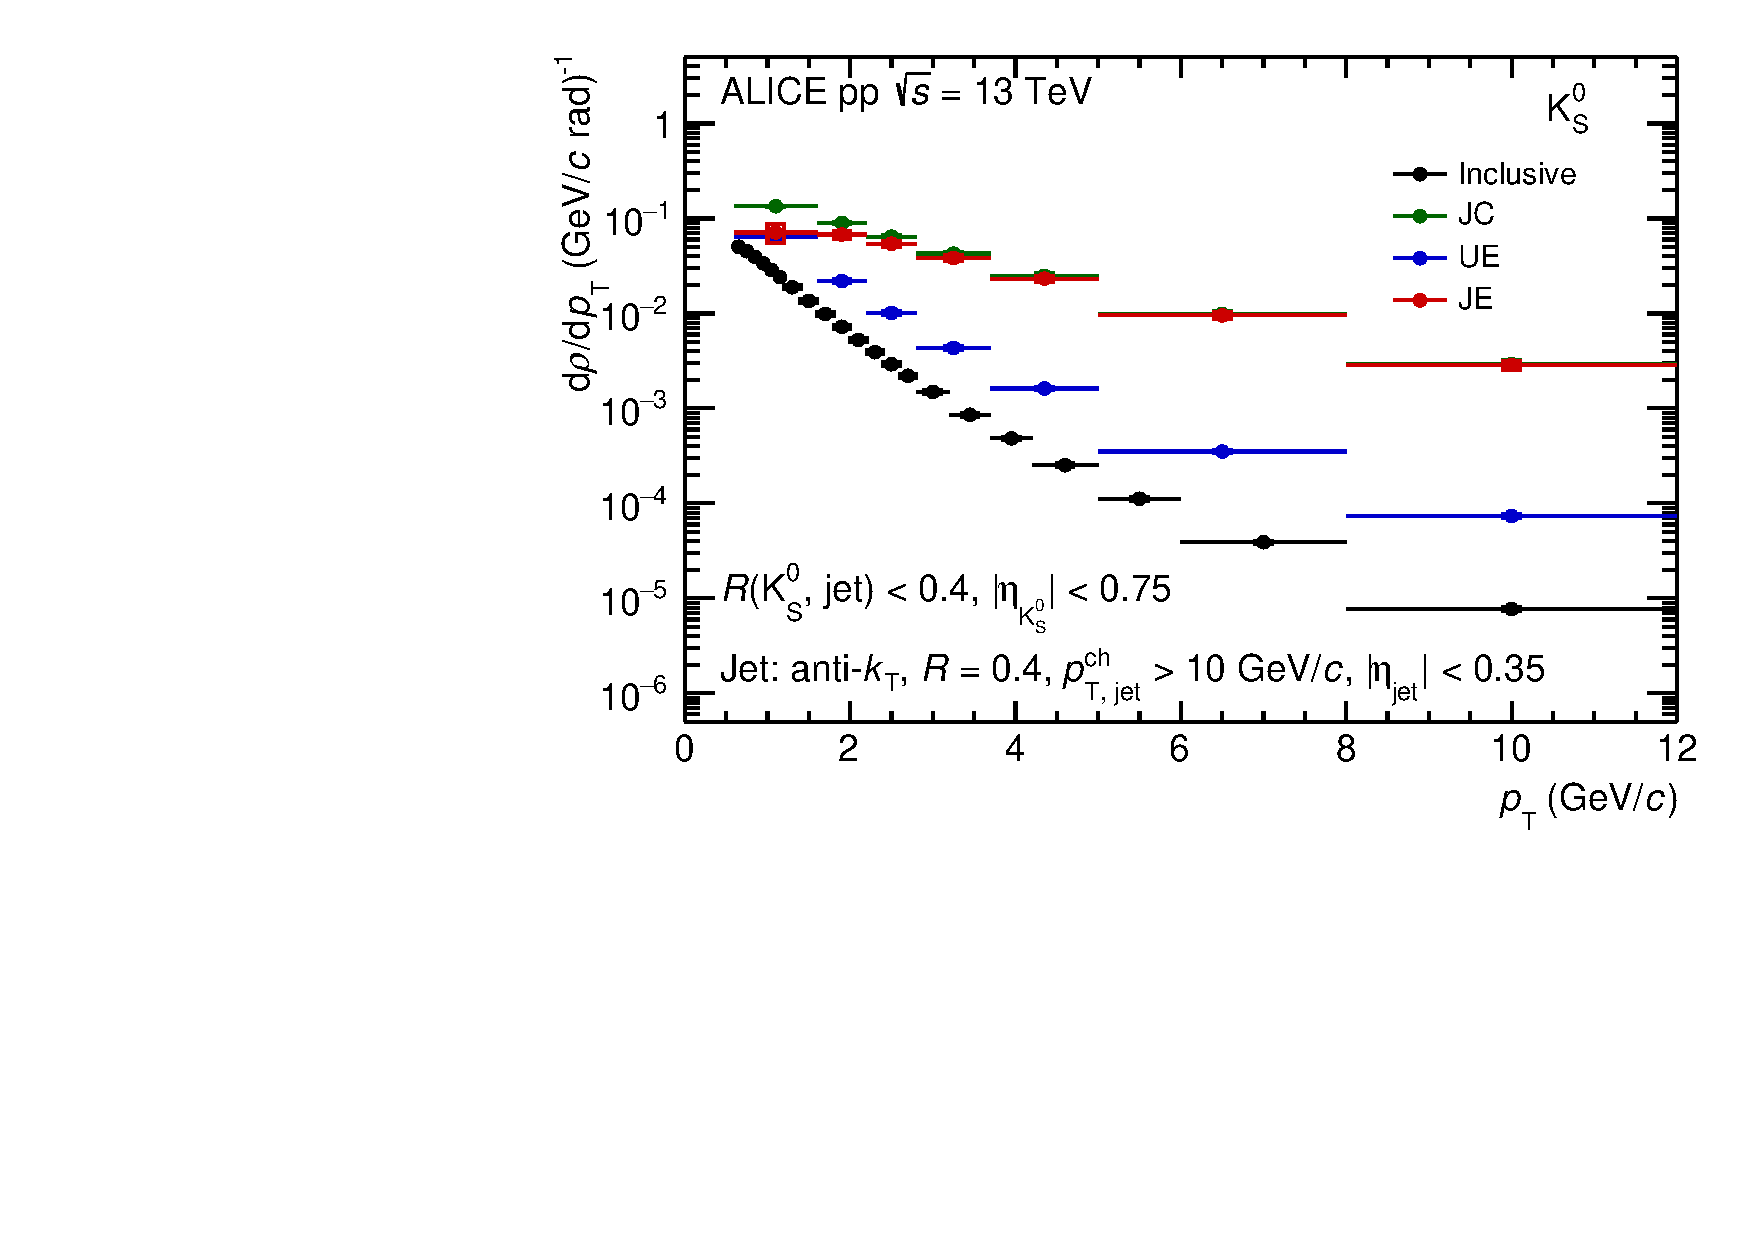
\includegraphics[width=.4\textwidth]{cf4_1}
		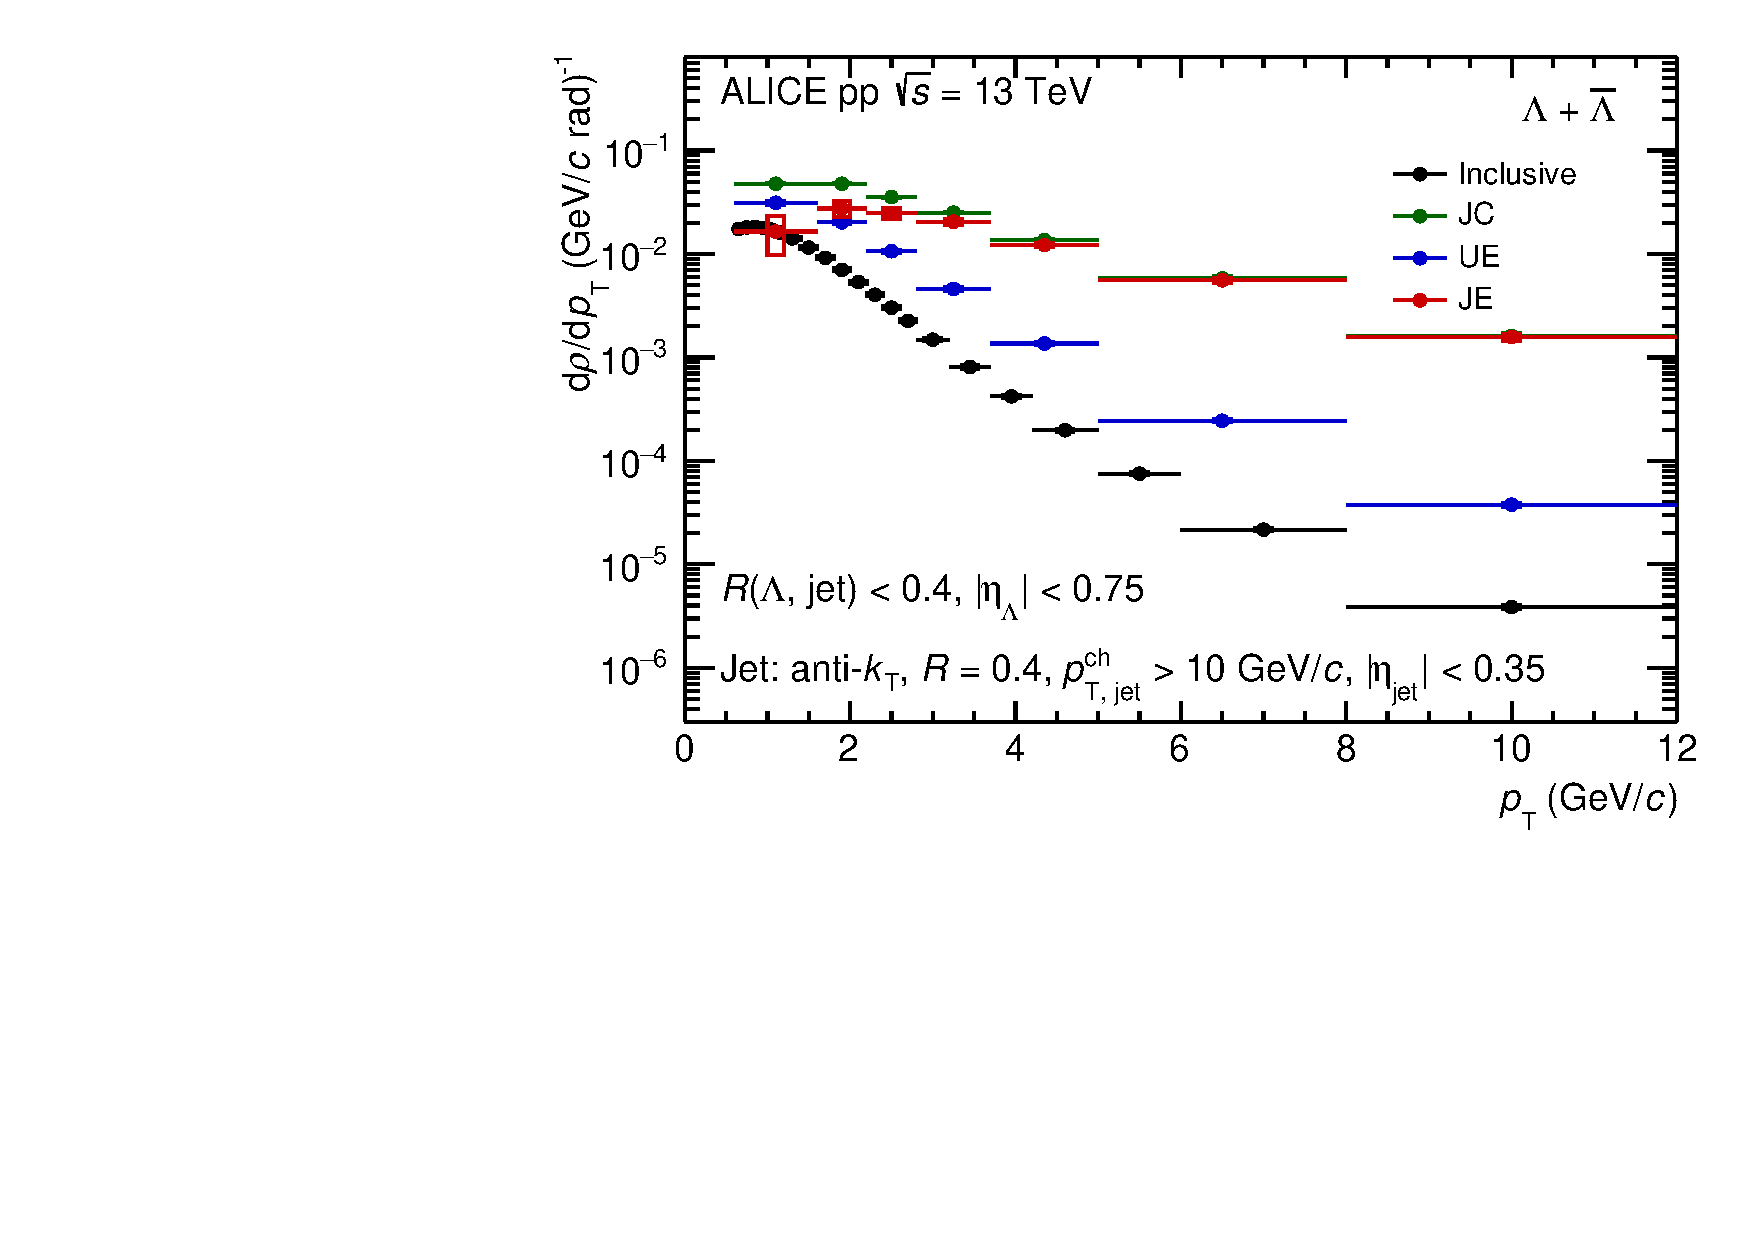
\includegraphics[width=.4\textwidth]{cf4_2}
		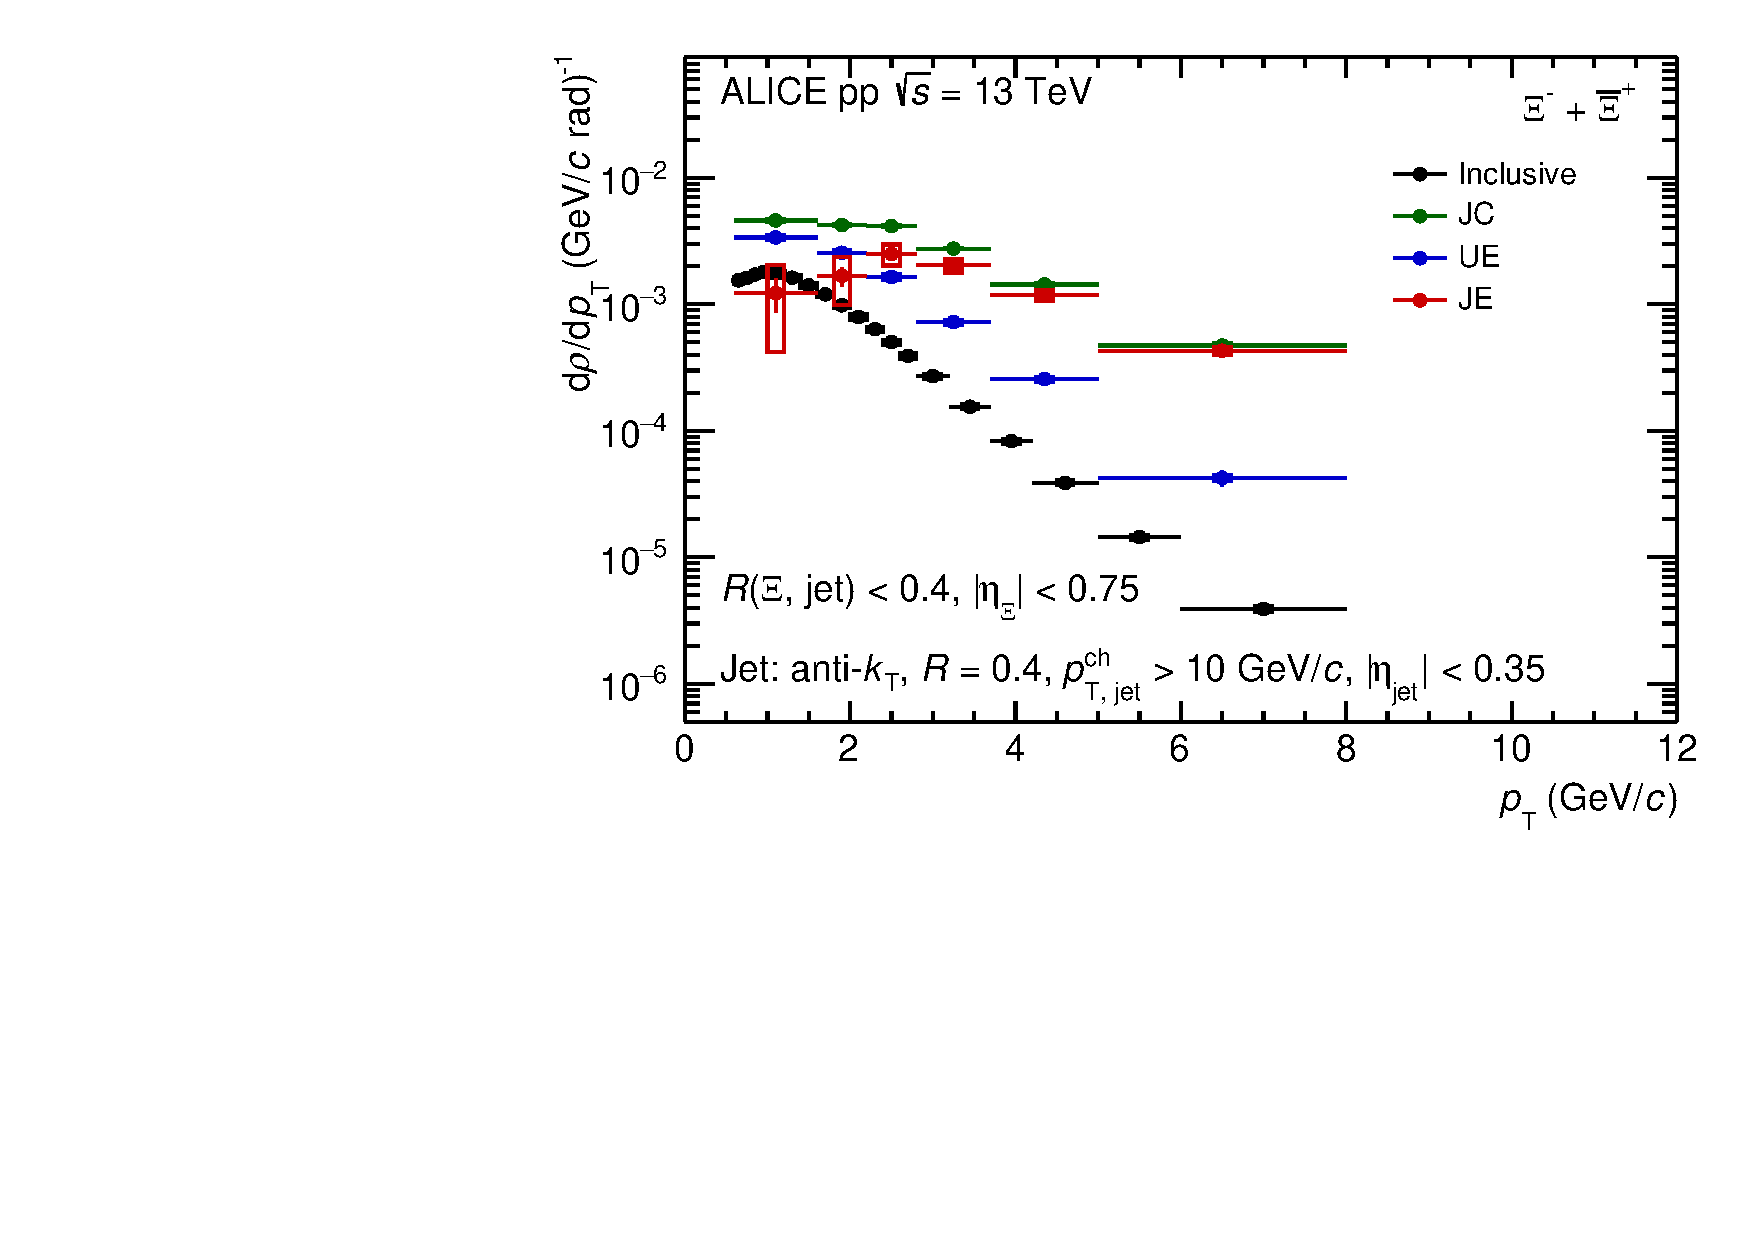
\includegraphics[width=.4\textwidth]{cf4_3}
		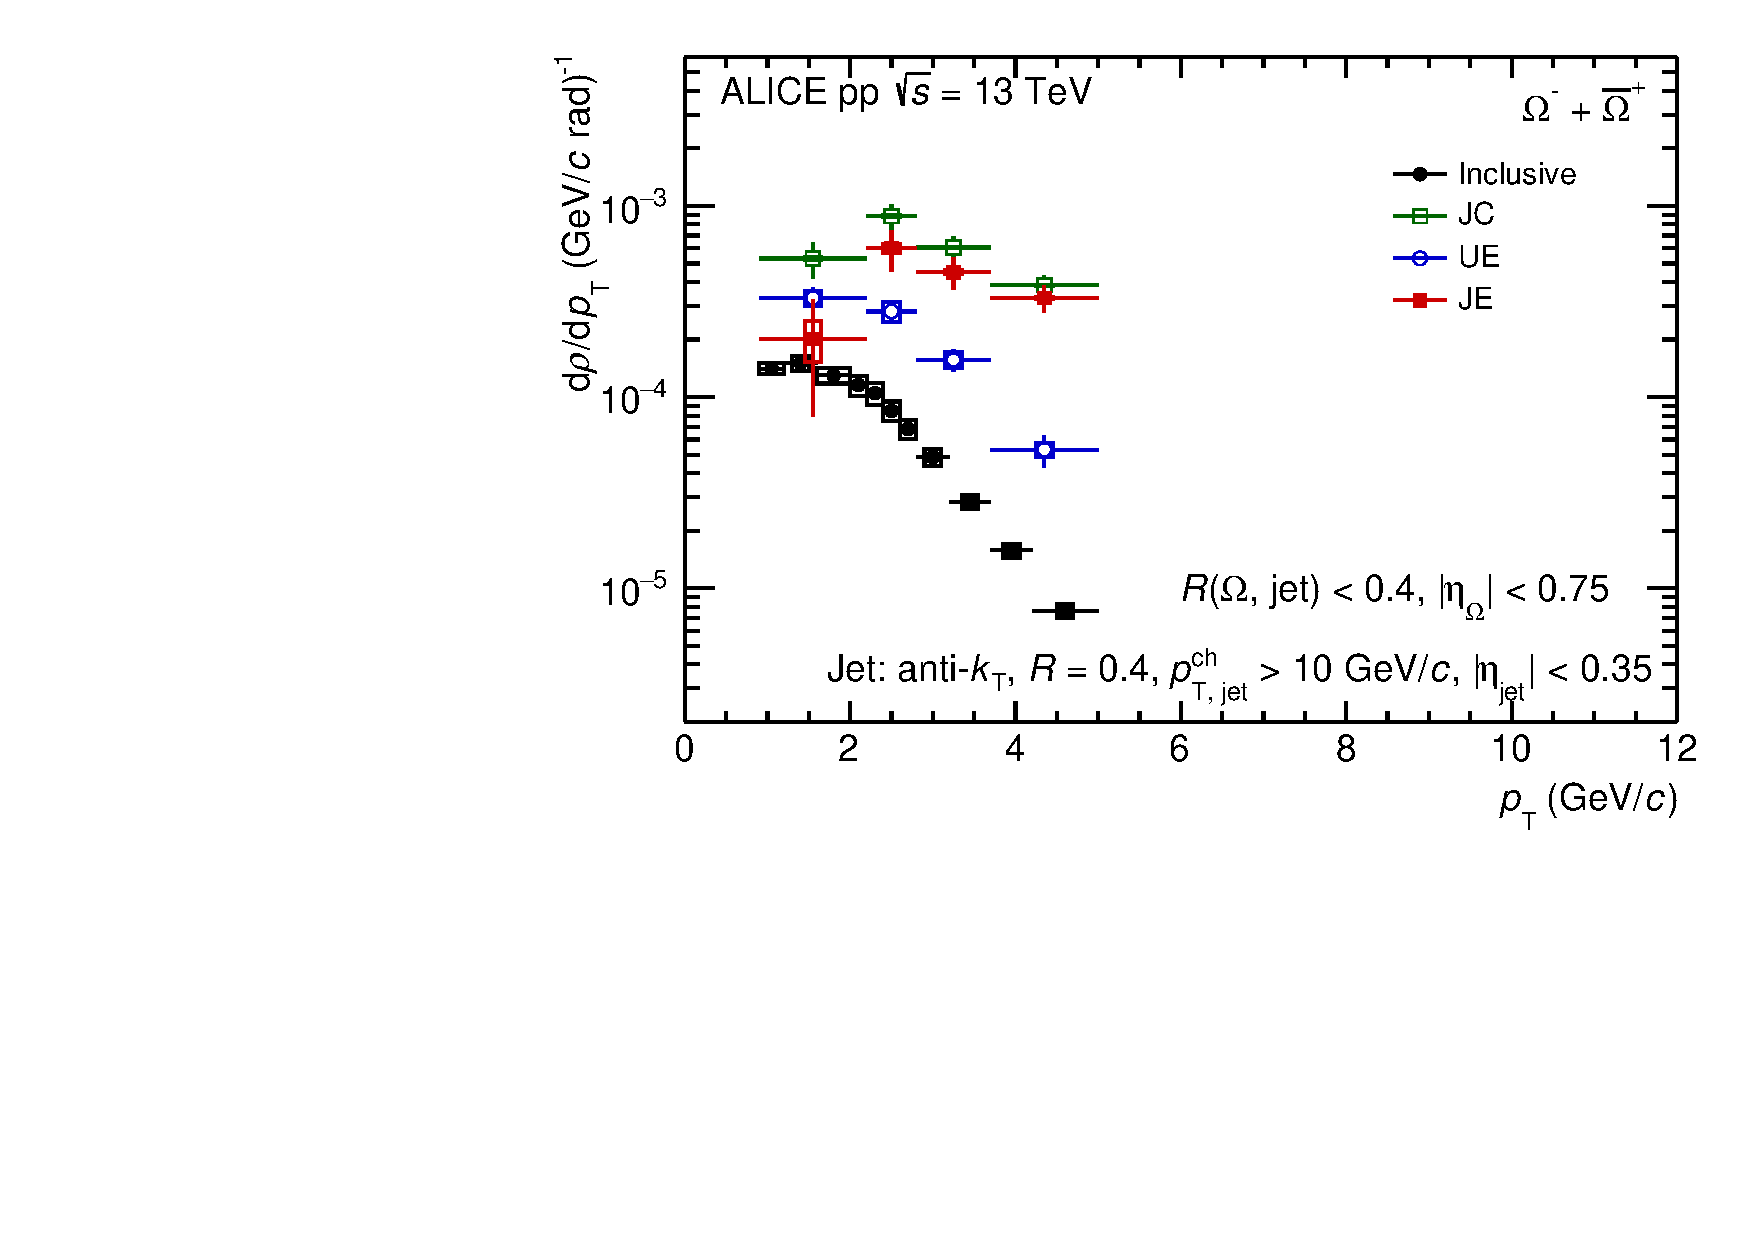
\includegraphics[width=.4\textwidth]{cf4_4}
	\end{center}
	\caption{$\pT$-differential density of strange hadrons }
	\label{fig:ppSpect}
\end{figure}
\begin{figure}[!ht]
	\begin{center}
		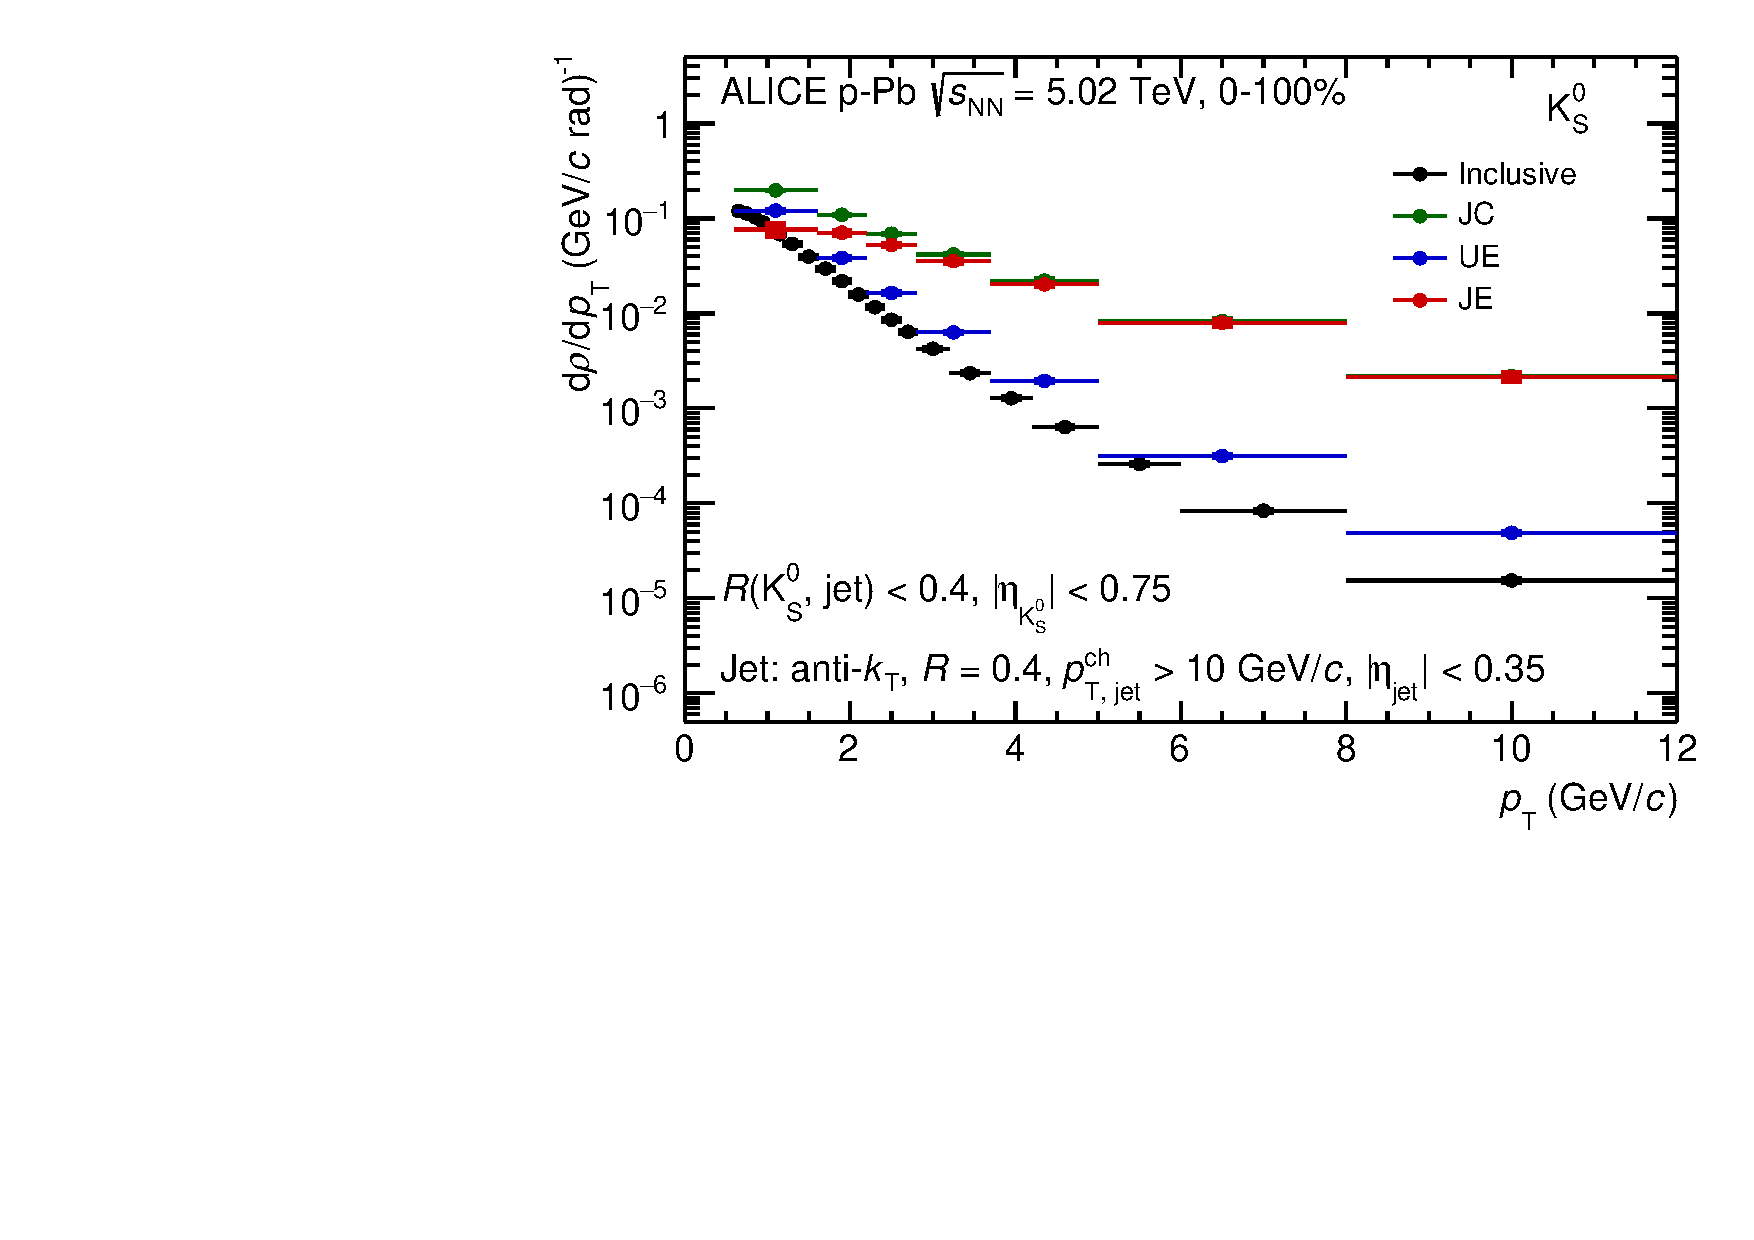
\includegraphics[width=.3\textwidth]{cf5_1}
		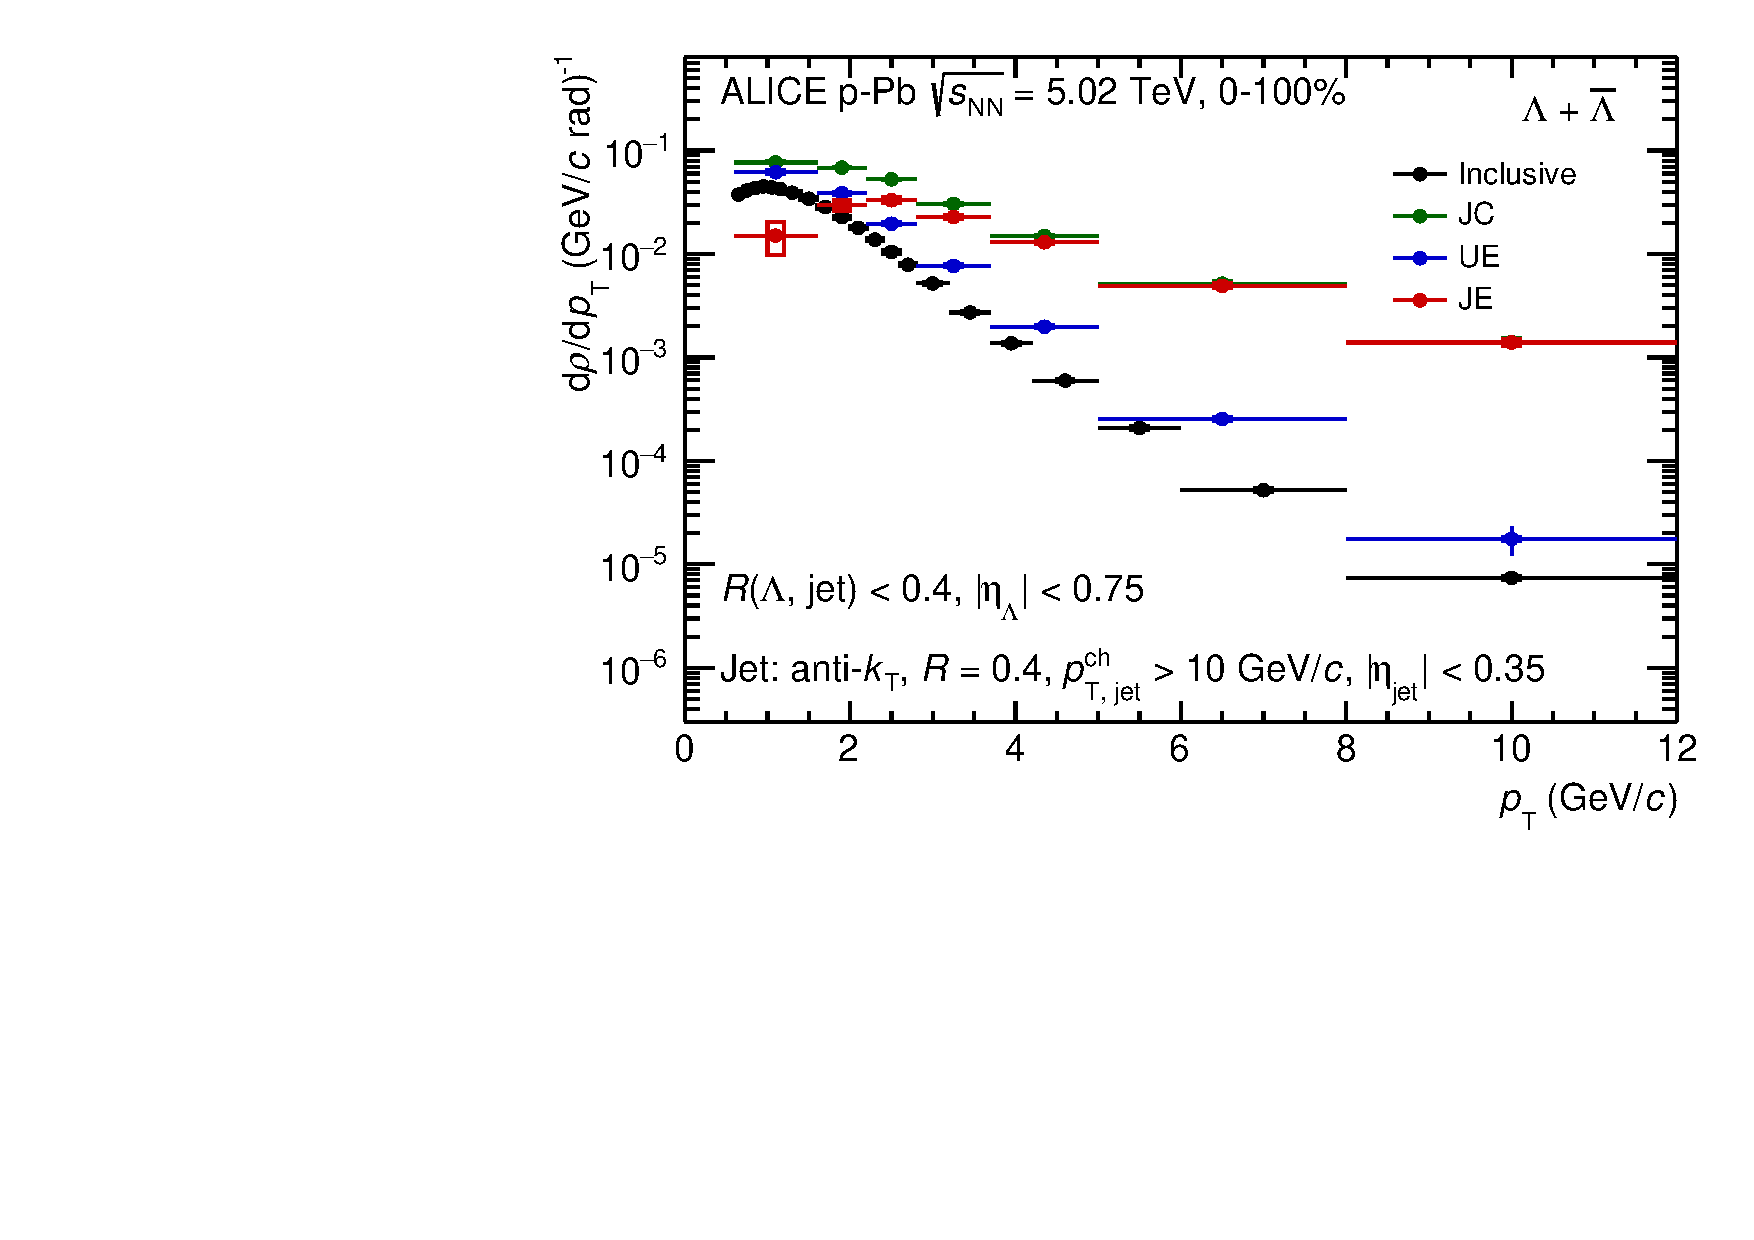
\includegraphics[width=.3\textwidth]{cf5_2}
		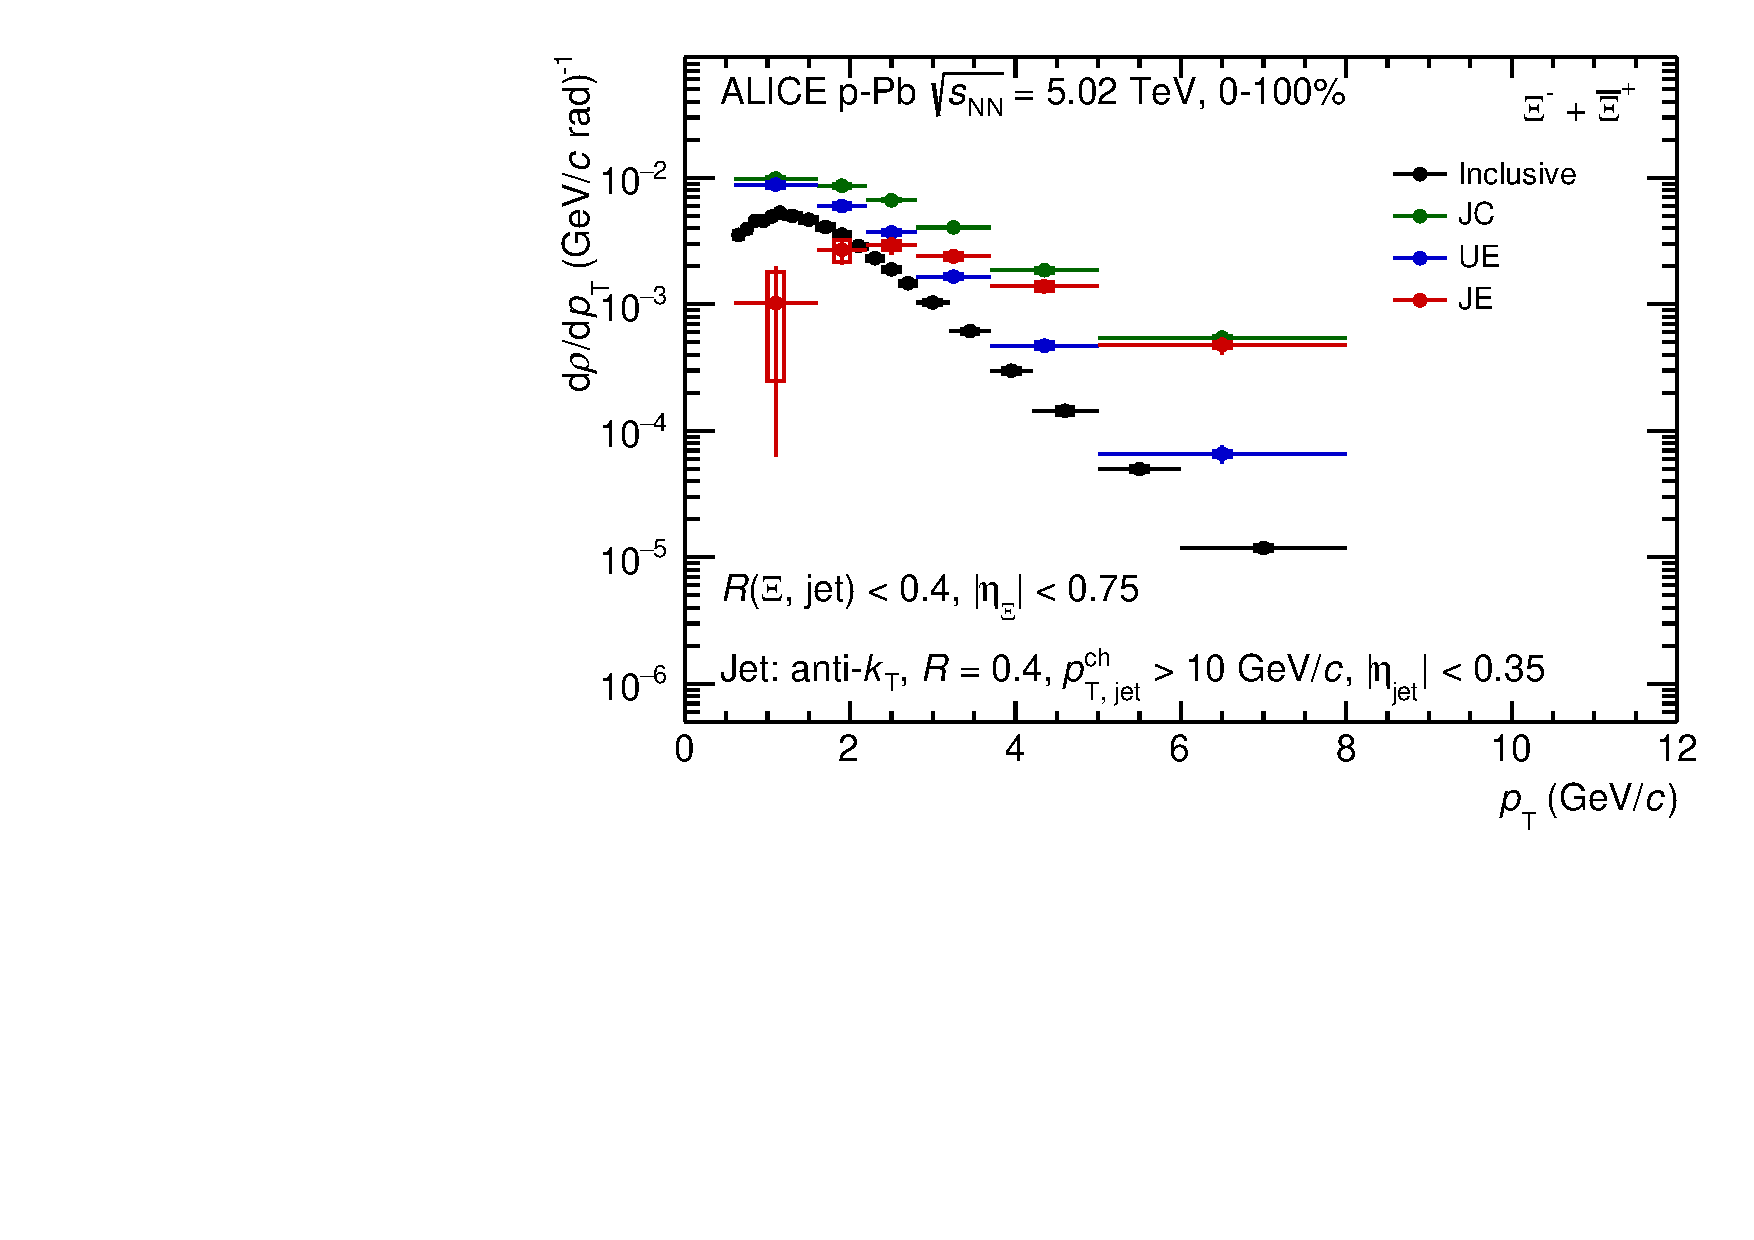
\includegraphics[width=.3\textwidth]{cf5_3}
		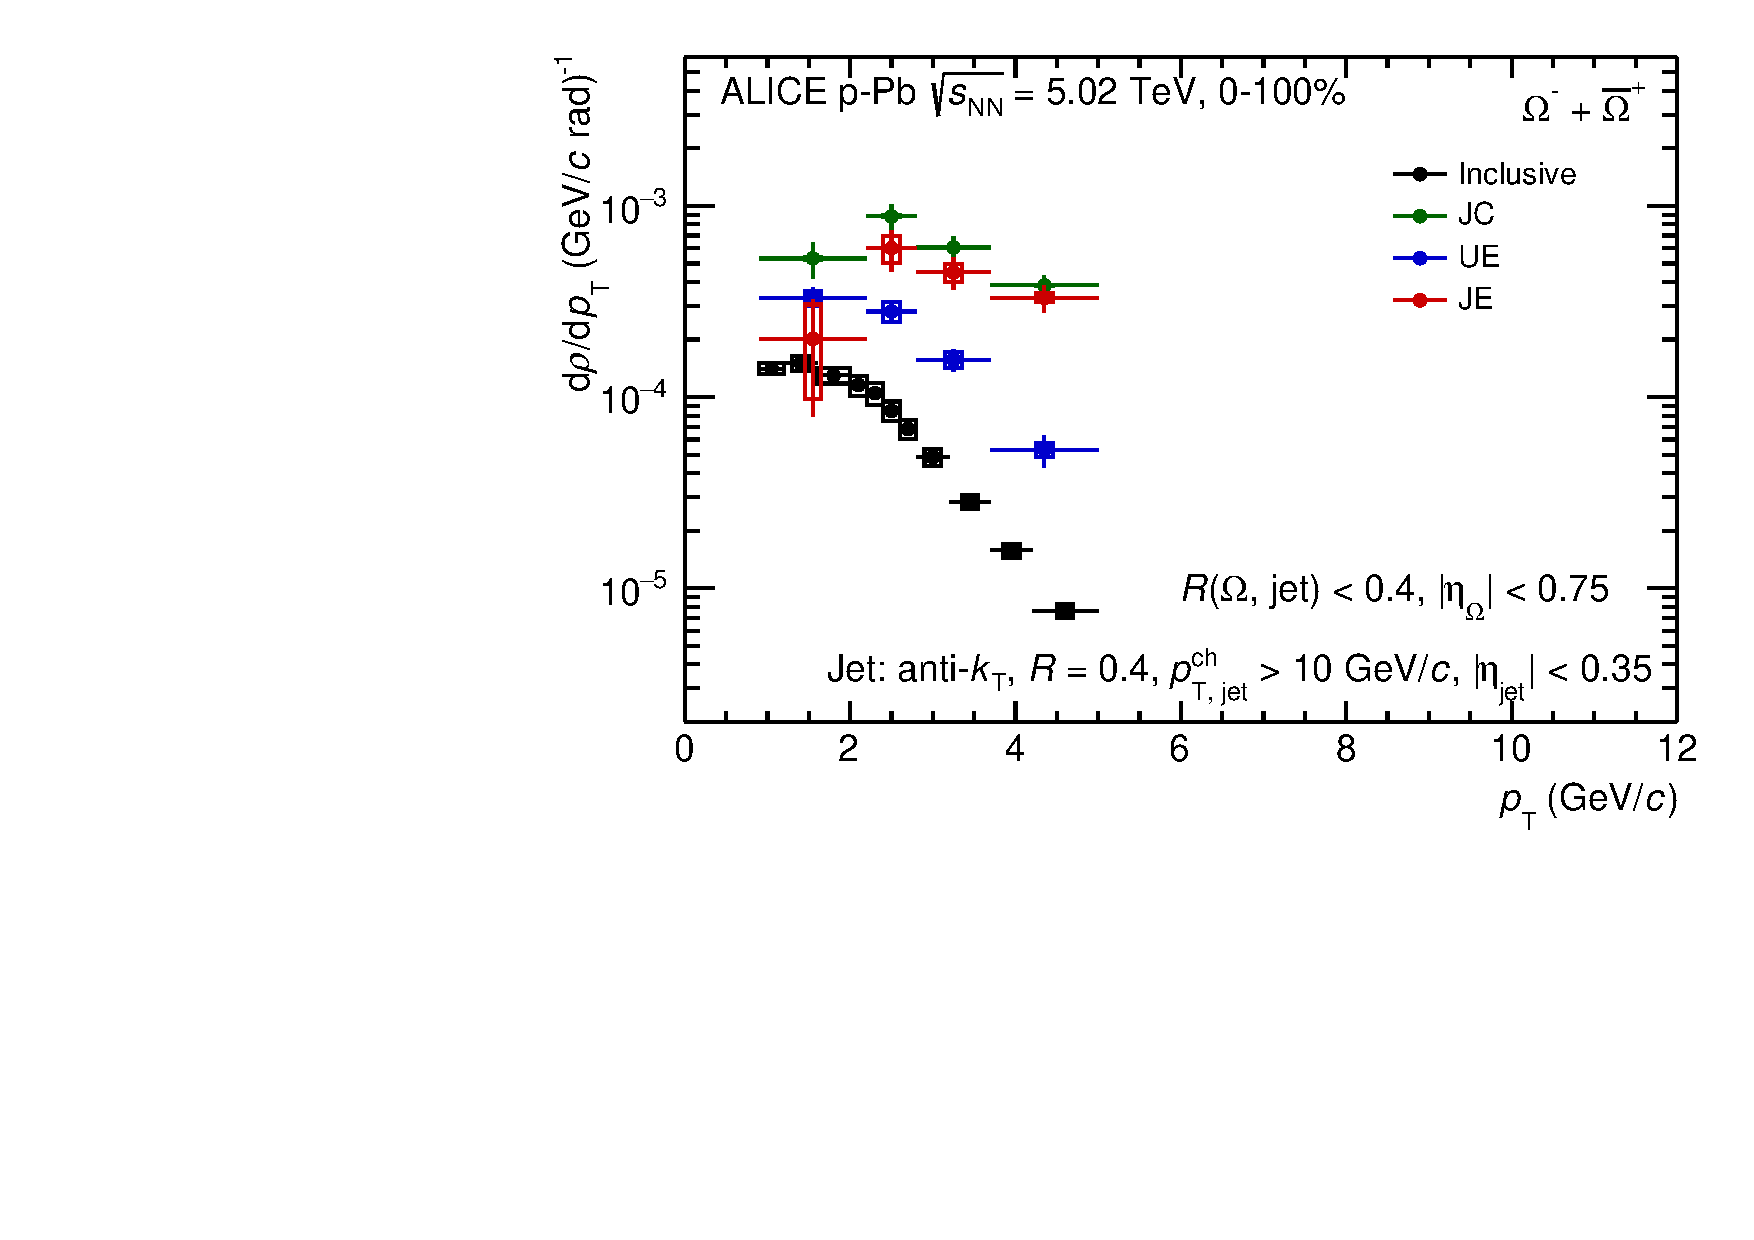
\includegraphics[width=.3\textwidth]{cf5_4}
		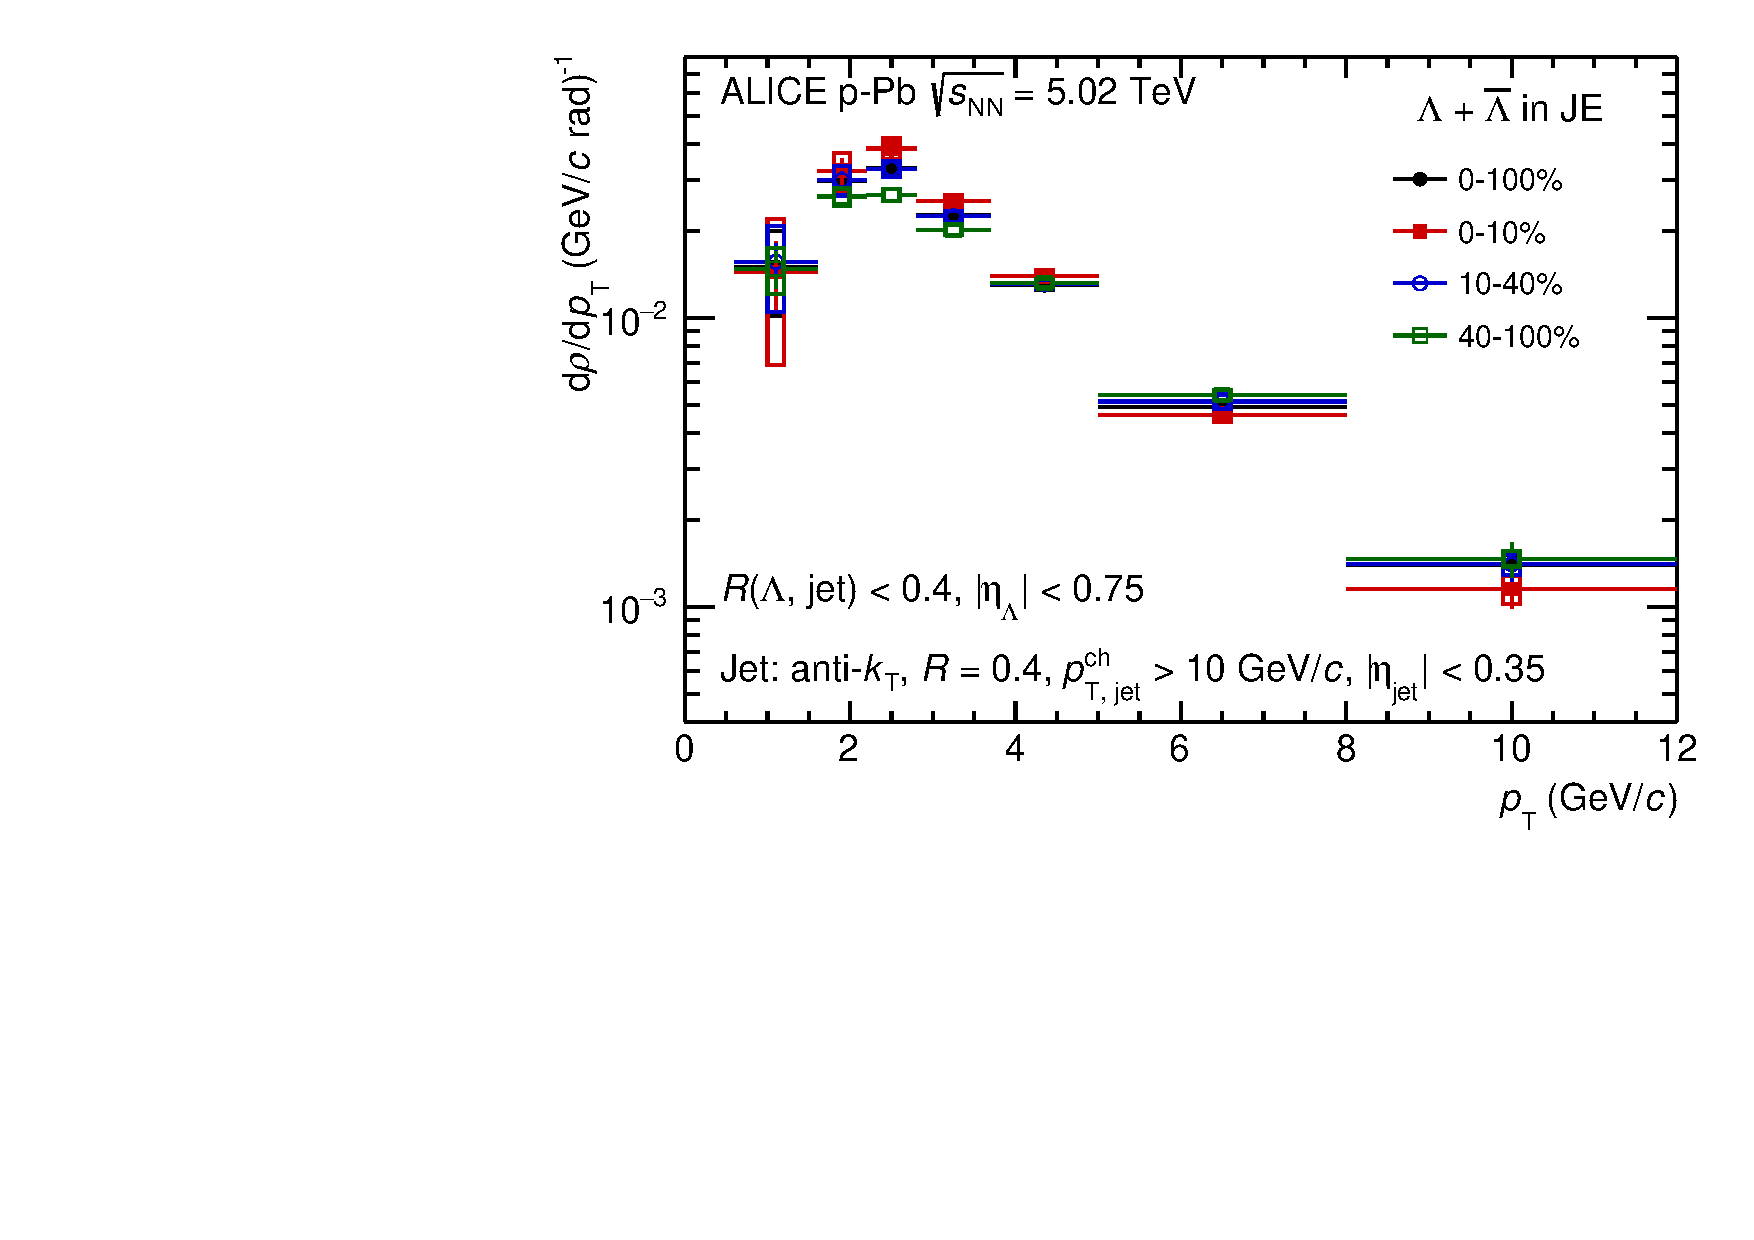
\includegraphics[width=.3\textwidth]{cf5_5}
		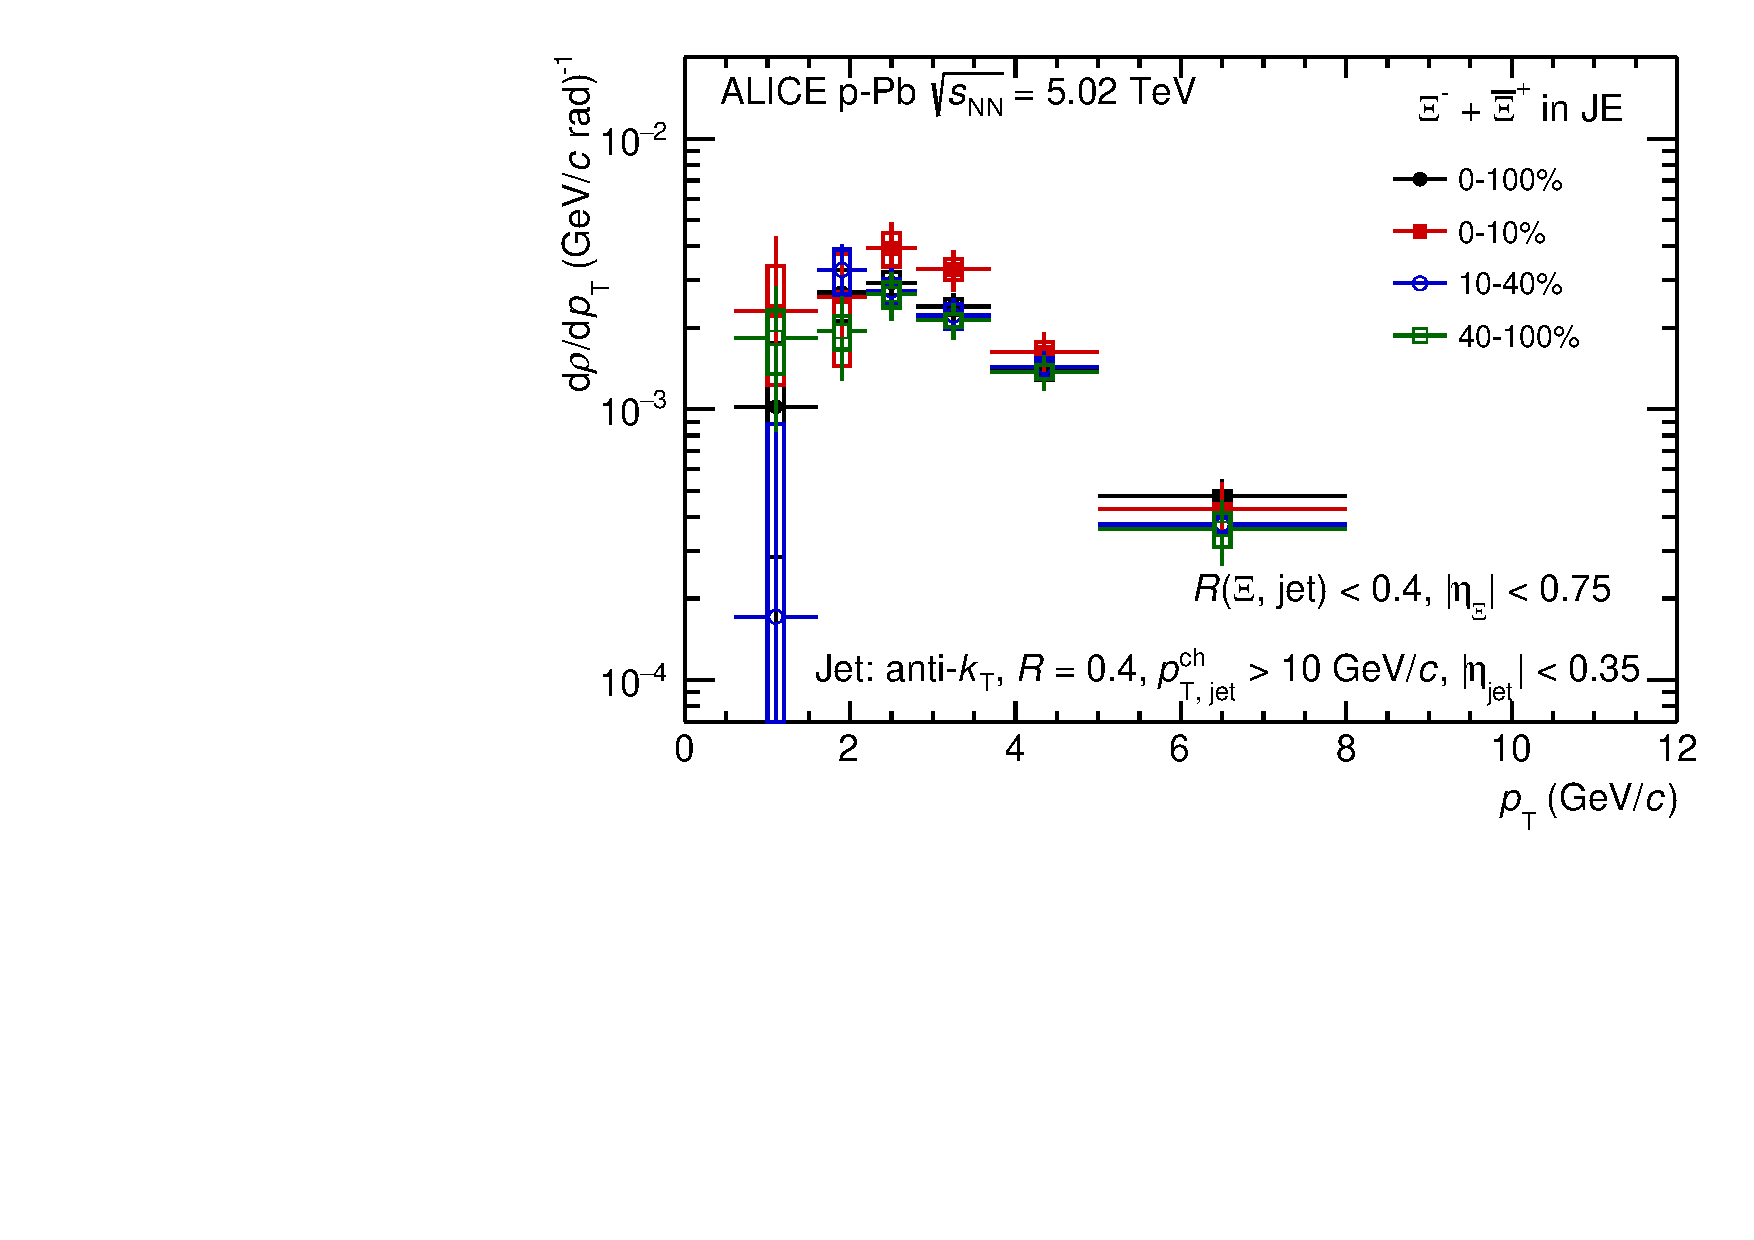
\includegraphics[width=.3\textwidth]{cf5_6}
	\end{center}
	\caption{$\pT$-differential density of strange hadrons }
	\label{fig:pPbSpect}
\end{figure}
\subsection{Baryon-to-meson and baryon-to-baryon ratios}
\label{subsec:ParRatios}



\subsection{Compare to models}
\label{subsec:ComToMod}
